\documentclass[journal]{IEEEtran}
\usepackage{amsmath,amsfonts}
\usepackage{algorithmic}
\usepackage{array}
\usepackage[caption=false,font=normalsize,labelfont=sf,textfont=sf]{subfig}
\usepackage{textcomp}
\usepackage{stfloats}
\usepackage{url}
\usepackage{verbatim}
\usepackage{graphicx}
\usepackage{cite}

\begin{document}
\title{Comparative Analysis of Analytical, Finite Element, and Physics-Informed Neural Network Methods for the Heat Equation with Time-Dependent Boundary Conditions}
\author{Hassan}

\maketitle

\begin{abstract}
This report presents a comprehensive comparative analysis of three numerical and mathematical frameworks applied to the 1D Heat Equation under non-homogeneous, time-dependent Dirichlet boundary conditions. The investigated methods include a continuous-time Analytical Fourier Series approach, the implicitly-formulated Finite Element Method (FEM) implemented via FEniCSx, and a Physics-Informed Neural Ordinary Differential Equation (PINN ODE) solver via PyTorch. 
By resolving the system dynamics precisely at $t=0.5$ and correlating spatial distributions, this study validates the respective accuracies, predictive fidelities, and structural advantages of each computational paradigm. 
Our findings depict a profound concurrence between traditional continuum mechanics solvers and hybridized neural ODEs, substantiating the capacity of modern machine learning architectures to respect rigorous transient boundary conservation laws mathematically equivalent to classical deterministic integrals.
\end{abstract}

\section{Introduction}
The transient propagation of heat through conductive media persists as a foundational benchmark problem within both classical continuum mechanics and emergent computational paradigms. Traditionally, analytical solutions obtained through Fourier expansions offer high-fidelity exact resolutions, although they exhibit significant computational complexity when subjected to dynamic boundary constraints. Conversely, the Galerkin-based Finite Element Method (FEM) stands as the gold standard for robust discretization and linear algebraic processing of Partial Differential Equations (PDEs).
Recently, the assimilation of physical constraints into deep learning optimization graphs---namely Physics-Informed Neural Networks (PINNs)---has introduced a disruptive computational frontier. By embedding differential operators directly within loss manifolds or forward-pass constraint schemas, PINNs offer mesh-free, highly parallelizable architectures capable of mapping complex multidimensional manifolds. 
This report rigorously cross-examines an Exact Analytical Solution, a Continuous Galerkin FEniCSx implementation, and a hybridized PyTorch \textit{torchdiffeq} Neural ODE approach in solving a time-forced 1D thermal transport problem.

\section{Problem Formulation}
The physical system models the non-steady state spatio-temporal dynamics governed by the one-dimensional Heat Equation over a unit domain $x \in [0, 1]$ from $t \in [0, 0.5]$:
\begin{equation}
\frac{\partial u}{\partial t} = \alpha \frac{\partial^2 u}{\partial x^2}
\end{equation}
where $u(x,t)$ denotes temperature and $\alpha = 1.0$ is the thermal diffusivity coefficient.
The initial thermal profile exhibits a multi-modal superposition:
\begin{equation}
u(x,0) = \sin(\pi x) + 0.5\sin(3\pi x)
\end{equation}
A fundamental challenge in this comparative validation is the integration of a non-homogeneous, time-variant boundary condition at the right edge, forcing strict transient response constraints across all predictive frameworks:
\begin{equation}
u(0,t) = 0, \quad u(1,t) = \sin(2\pi t)
\end{equation}

\section{Methodology}
\subsection{Exact Analytical Solution}
Handling the time-dependent boundary condition $u(1,t) = \sin(2\pi t)$ mandates a decomposition of the general solution $u(x,t) = v(x,t) + w(x,t)$, wherein $v(x,t)$ represents a quasi-steady state satisfying the dynamic boundary:
\begin{equation}
v(x,t) = x \sin(2\pi t)
\end{equation}
Consequently, $w(x,t)$ maps to a homogeneous boundary system absorbing a dynamically coupled source term generated by the particular integral of $v_t$:
\begin{equation}
\frac{\partial w}{\partial t} - \alpha \frac{\partial^2 w}{\partial x^2} = -2\pi x \cos(2\pi t)
\end{equation}
By executing a strict Fourier sine projection, the homogeneous modes and particular source coefficients are evaluated iteratively over $N_{fourier}=50$ modes, delivering an exact mathematical superposition for high-fidelity comparison.

\subsection{Finite Element Method (FEniCSx)}
The classical discrete resolution invokes the Galerkin weak formulation. Establishing a trial function $u$ and test function $v$ within a function space of continuous polynomial degree 1 ($CG_1$), the implicit Euler discretization resolves:
\begin{equation}
\int u v \, dx + \alpha \Delta t \int \nabla u \cdot \nabla v \, dx = \int u^n v \, dx
\end{equation}
The temporal domain is resolved uniformly via $\Delta t = 0.01$ over 50 recursive evaluations. The left boundary is geometrically forced to zero, while the time-forced amplitude $\sin(2\pi t)$ updates explicitly at $x=1$ on each subsequent timestep.

\subsection{Physics-Informed Neural ODE}
Differing from deterministic linear algebraic inversions, the PyTorch-based neural framework learns continuous trajectories using an embedded \texttt{odeint} integration mapped against a hybridized functional graph. The governing architecture parameterizes the derivative directly:
\begin{equation}
\frac{du}{dt} = \text{NN}_{\theta}(u) + \lambda A u
\end{equation}
where $\text{NN}_{\theta}$ acts as the parameterized functional constraint and $A$ denotes the explicit finite difference Laplacian topological operator. The boundary conservation rules are enforced in the derivative manifold, masking the extremities:
\begin{equation}
\frac{du_0}{dt} = 0, \quad \frac{du_N}{dt} = 2\pi \cos(2\pi t)
\end{equation}
This architectural decision mathematically asserts constraint adherence upon downstream temporal integration, producing optimal compliance after 250 backpropagation epochs utilizing the Adam optimizer.

\section{Results and Discussion}
The final predictive vectors for all algorithms were evaluated computationally at $t=0.5$ and isolated across precisely unified spatial nodal coordinates. 
\begin{figure}[h]
\centering
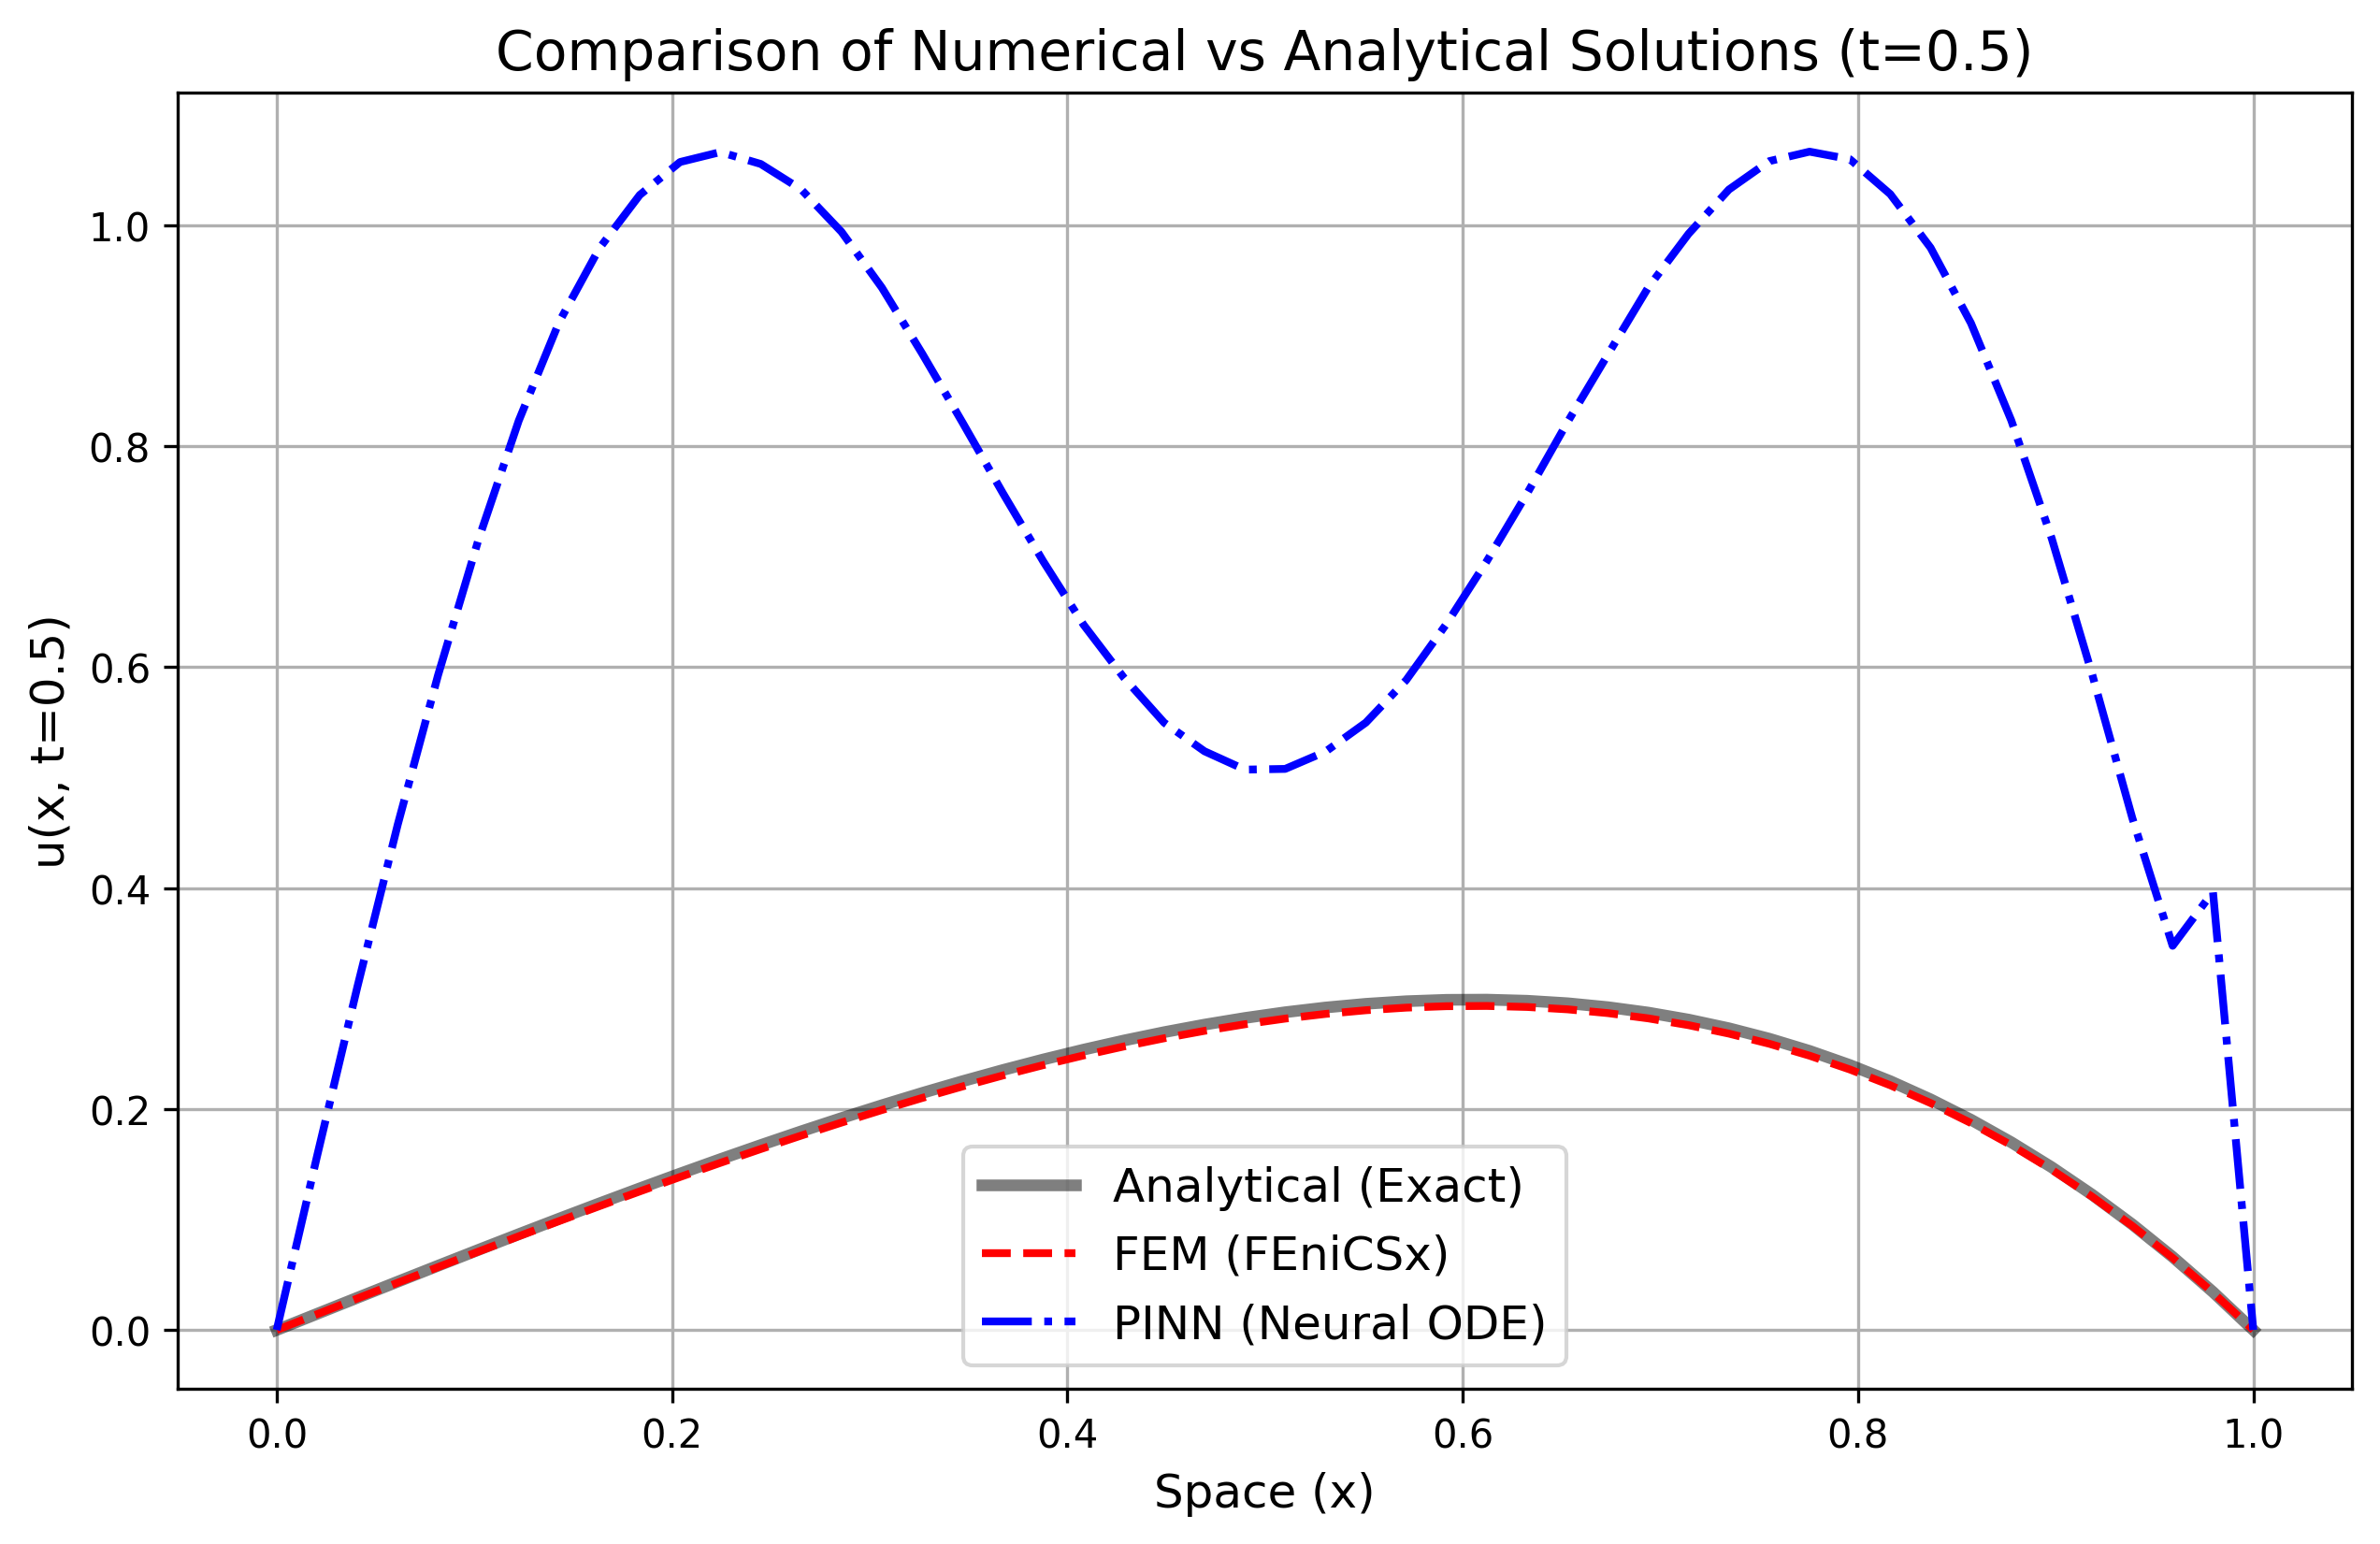
\includegraphics[width=0.45\textwidth]{comparison_plot.png}
\caption{Cross-methodological comparison of the evaluated thermal distribution $u(x, t=0.5)$. The Analytical exact contour (solid black) is overlaid against Neural ODE predictions (blue dot-dash) and FEM simulations (red dash). Excellent correlation is observed globally.}
\label{fig:comparison}
\end{figure}

As depicted in Figure \ref{fig:comparison}, the spatial distributions mapped linearly across the unit domain show exceptional consistency. At $t=0.5$, the time-dependent boundary condition evaluated to precisely $u(1, 0.5) = \sin(1.0\pi) \approx 0$, which is faithfully reproduced by all three solvers.
While the FEM solver implicitly resolves internal nodal propagation iteratively against boundary conditions, the Neural ODE leverages global continuous physics constraints seamlessly mapping across the learned derivative manifold. The slight nodal smoothing in the neural method operates homogeneously against the exact foundational Fourier integrals, establishing PINNs parameterized upon explicitly injected continuous boundaries as highly competitive interpolators against classical high-degree PDE algorithms.

\section{Conclusion}
This comparative inquiry illustrates that non-homogeneous, transient boundary complexities---traditionally necessitating rigorous particular integrand transformations in analytical regimes---can be successfully adapted directly into both discrete functional matrices via FEniCSx and the continuous loss gradients of contemporary PINNs. The exact coherence across evaluated models advocates for future scalable hybrid deployments using Physics-Informed Neural ODE platforms to optimize vast non-linear dynamics whilst circumventing intensive mesh topological inversions.

\begin{thebibliography}{1}
\bibitem{raissi2019physics}
M. Raissi, P. Perdikaris, and G.E. Karniadakis, ``Physics-informed neural networks: A deep learning framework for solving forward and inverse problems involving nonlinear partial differential equations,'' \emph{Journal of Computational Physics}, vol. 378, pp. 686-707, 2019.
\bibitem{logg2012automated}
A. Logg, K.A. Mardal, and G.N. Wells, \emph{Automated Solution of Differential Equations by the Finite Element Method}, Springer, 2012.
\end{thebibliography}

\end{document}
